


\tikzset{every picture/.style={line width=0.75pt}} %set default line width to 0.75pt        

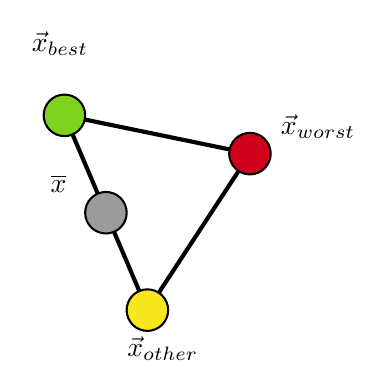
\begin{tikzpicture}[x=0.75pt,y=0.75pt,yscale=-1,xscale=1]
%uncomment if require: \path (0,914); %set diagram left start at 0, and has height of 914

%Straight Lines [id:da8438979087196363] 
\draw [line width=1.5]    (277.21,85.73) -- (366.59,104.19) ;
%Straight Lines [id:da20469279023180365] 
\draw [line width=1.5]    (317.18,179.58) -- (277.21,85.73) ;
%Straight Lines [id:da8334212569541255] 
\draw [line width=1.5]    (317.18,179.58) -- (366.59,104.19) ;
%Shape: Circle [id:dp35373016991770023] 
\draw  [fill={rgb, 255:red, 126; green, 211; blue, 33 }  ,fill opacity=1 ] (268.01,89.65) .. controls (265.85,84.57) and (268.21,78.7) .. (273.29,76.53) .. controls (278.37,74.37) and (284.25,76.73) .. (286.41,81.81) .. controls (288.57,86.9) and (286.21,92.77) .. (281.13,94.93) .. controls (276.05,97.1) and (270.17,94.73) .. (268.01,89.65) -- cycle ;
%Shape: Circle [id:dp40627430744057724] 
\draw  [fill={rgb, 255:red, 208; green, 2; blue, 27 }  ,fill opacity=1 ] (357.39,108.1) .. controls (355.22,103.02) and (357.59,97.15) .. (362.67,94.99) .. controls (367.75,92.82) and (373.62,95.19) .. (375.79,100.27) .. controls (377.95,105.35) and (375.59,111.22) .. (370.51,113.39) .. controls (365.43,115.55) and (359.55,113.19) .. (357.39,108.1) -- cycle ;
%Shape: Circle [id:dp7608960793687913] 
\draw  [fill={rgb, 255:red, 248; green, 231; blue, 28 }  ,fill opacity=1 ] (307.98,183.49) .. controls (305.82,178.41) and (308.18,172.54) .. (313.26,170.38) .. controls (318.34,168.21) and (324.22,170.58) .. (326.38,175.66) .. controls (328.54,180.74) and (326.18,186.61) .. (321.1,188.78) .. controls (316.02,190.94) and (310.14,188.58) .. (307.98,183.49) -- cycle ;
%Shape: Circle [id:dp5171429606236433] 
\draw  [fill={rgb, 255:red, 155; green, 155; blue, 155 }  ,fill opacity=1 ] (287.99,136.57) .. controls (285.83,131.49) and (288.2,125.62) .. (293.28,123.45) .. controls (298.36,121.29) and (304.23,123.65) .. (306.4,128.74) .. controls (308.56,133.82) and (306.19,139.69) .. (301.11,141.85) .. controls (296.03,144.02) and (290.16,141.65) .. (287.99,136.57) -- cycle ;

% Text Node
\draw (260,44) node [anchor=north west][inner sep=0.75pt]   [align=left] {$\displaystyle \vec{x}_{best}$};
% Text Node
\draw (380,84) node [anchor=north west][inner sep=0.75pt]   [align=left] {$\displaystyle \vec{x}_{worst}$};
% Text Node
\draw (306,191) node [anchor=north west][inner sep=0.75pt]   [align=left] {$\displaystyle \vec{x}_{other}$};
% Text Node
\draw (269,113) node [anchor=north west][inner sep=0.75pt]   [align=left] {$\displaystyle \overline{x}$};


\end{tikzpicture}